\documentclass[journal,12pt]{IEEEtran}
%

\usepackage{setspace}
\usepackage{textcomp}
\usepackage{gensymb}
\singlespacing
\usepackage{hyperref}
\usepackage{amsmath}
\usepackage{amsthm}
\usepackage{txfonts}
\usepackage{cite}
\usepackage{enumitem}
\usepackage{mathtools}
\usepackage{listings}
    \usepackage{color}                                            %%
    \usepackage{array}                                            %%
    \usepackage{longtable}                                        %%
    \usepackage{calc}                                             %%
    \usepackage{multirow}                                         %%
    \usepackage{hhline}                                           %%
    \usepackage{ifthen}                                           %%
  %optionally (for landscape tables embedded in another document): %%
    \usepackage{lscape}     
\usepackage{multicol}
\usepackage{chngcntr}
\usepackage[center]{caption}
\renewcommand\thesection{\arabic{section}}
\renewcommand\thesubsection{\thesection.\arabic{subsection}}
\renewcommand\thesubsubsection{\thesubsection.\arabic{subsubsection}}

\renewcommand\thesectiondis{\arabic{section}}
\renewcommand\thesubsectiondis{\thesectiondis.\arabic{subsection}}
\renewcommand\thesubsubsectiondis{\thesubsectiondis.\arabic{subsubsection}}

% correct bad hyphenation here
\hyphenation{op-tical net-works semi-conduc-tor}
\def\inputGnumericTable{}                                 %%

\lstset{
%language=C,
frame=single, 
breaklines=true,
columns=fullflexible
}

\begin{document}
%


\newtheorem{theorem}{Theorem}[section]
\newtheorem{problem}{Problem}
\newtheorem{proposition}{Proposition}[section]
\newtheorem{lemma}{Lemma}[section]
\newtheorem{corollary}[theorem]{Corollary}
\newtheorem{example}{Example}[section]
\newtheorem{definition}[problem]{Definition}
\newcommand{\BEQA}{\begin{eqnarray}}
\newcommand{\EEQA}{\end{eqnarray}}
\newcommand{\define}{\stackrel{\triangle}{=}}
\bibliographystyle{IEEEtran}
\providecommand{\mbf}{\mathbf}
\providecommand{\pr}[1]{\ensuremath{\Pr\left(#1\right)}}
\providecommand{\qfunc}[1]{\ensuremath{Q\left(#1\right)}}
\providecommand{\sbrak}[1]{\ensuremath{{}\left[#1\right]}}
\providecommand{\lsbrak}[1]{\ensuremath{{}\left[#1\right.}}
\providecommand{\rsbrak}[1]{\ensuremath{{}\left.#1\right]}}
\providecommand{\brak}[1]{\ensuremath{\left(#1\right)}}
\providecommand{\lbrak}[1]{\ensuremath{\left(#1\right.}}
\providecommand{\rbrak}[1]{\ensuremath{\left.#1\right)}}
\providecommand{\cbrak}[1]{\ensuremath{\left\{#1\right\}}}
\providecommand{\lcbrak}[1]{\ensuremath{\left\{#1\right.}}
\providecommand{\rcbrak}[1]{\ensuremath{\left.#1\right\}}}
\theoremstyle{remark}
\newtheorem{rem}{Remark}
\newcommand{\sgn}{\mathop{\mathrm{sgn}}}
\providecommand{\abs}[1]{\left\vert#1\right\vert}
\providecommand{\res}[1]{\Res\displaylimits_{#1}} 
\providecommand{\norm}[1]{\left\lVert#1\right\rVert}
\providecommand{\mtx}[1]{\mathbf{#1}}
\providecommand{\mean}[1]{E\left[ #1 \right]}
\providecommand{\fourier}{\overset{\mathcal{F}}{ \rightleftharpoons}}
\providecommand{\system}{\overset{\mathcal{H}}{ \longleftrightarrow}}
\newcommand{\solution}{\noindent \textbf{Solution: }}
\newcommand{\cosec}{\,\text{cosec}\,}
\providecommand{\dec}[2]{\ensuremath{\overset{#1}{\underset{#2}{\gtrless}}}}
\newcommand{\myvec}[1]{\ensuremath{\begin{pmatrix}#1\end{pmatrix}}}
\newcommand{\cmyvec}[1]{\ensuremath{\begin{pmatrix*}[c]#1\end{pmatrix*}}}
\newcommand{\mydet}[1]{\ensuremath{\begin{vmatrix}#1\end{vmatrix}}}
\newcommand{\proj}[2]{\textbf{proj}_{\vec{#1}}\vec{#2}}
\let\StandardTheFigure\thefigure
\let\vec\mathbf
\title{EE5600 - Introduction to AI \& ML\\Assignment 1}
\author{Virendra Patil\\AI20MTECH01003}	
\maketitle
%\renewcommand{\thefigure}{\theenumi}
\renewcommand{\thetable}{\theenumi}
\begin{abstract}
Given the vector coordinates of the angular points of the triangle, we need to find the area of the triangle. In vector space, the area of parallelogram formed by any two vectors is given by the magnitude of the cross product of those two vectors. The area of traingle whose two sides are represented by vectors is nothing but half the area of parallelogram formed by the respective vectors. In essence, area of triangle whose two sides are represented by two vectors u and v is given by $\frac{1}{2} \times ||(u \times v)||$, where "$u \times v$" represents cross product of two vectors. The python implementation of the said method is available at  \href{https://github.com/virendra-patil/EE5600-Intro-to-AI-ML/tree/main/Assignment_1}{\emph{https://github.com/virendra-patil/EE5600-Intro-to-AI-ML/tree/main/Assignment\_1}}.
\end{abstract}
%
%Download all python and latex codes from 
%
%\begin{lstlisting}

%\end{lstlisting}
%
\section{Problem Statement}

Vector2, Example II, Problem 4: Find the area of the triangle whose coordinates of angular points are respectively,\\\\ $\myvec{a\\b+c}$, $\myvec{a\\b-c}$ and $\myvec{-a\\c}$.

%\renewcommand{\theequation}{\theenumi}
%\begin{enumerate}[label=\thesection.\arabic*.,ref=\thesection.\theenumi]
%\numberwithin{equation}{enumi}
%\item 

\section{Solution}
We solve the above stated problem in two steps. First, we find two vectors representing sides of the given triangle. In second step we calculate area of parallelogram and halve it to obtain the area of triangle. Initially we propose a generalise solution and extend it by solving the same problem using example coordinates.\\\\
Step I:\\\\
Let,
\begin{align}
\vec{X} = \myvec{a\\b+c}, \text{ } \vec{Y} = \myvec{a\\b-c} \text{ and } \vec{Z} = \myvec{-a\\c}
\label{eq1}
\end{align}
Rewriting X, Y and Z as product of a matrix and a vector, we get,\\
\begin{align}
\begin{split}
\vec{X} & = \Bigg[\myvec{1&0&0\\0&1&1}\myvec{a\\b\\c}\Bigg] \\
\vec{Y} & = \Bigg[\myvec{1&0&0\\0&1&-1}\myvec{a\\b\\c}\Bigg] \\
\vec{Z} & = \Bigg[\myvec{-1&0&0\\0&0&1}\myvec{a\\b\\c}\Bigg] 
\end{split}
\label{eq2}
\end{align}
As X, Y and Z represent coordinates of angular points of the triangle, by vector calculus X-Y, Y-Z and X-Z would represent the sides of the triangle. To calculate area of triangle we need any two sides. Here we consider X-Y and Y-Z.\\
\begin{align}
\begin{split}
\vec{X-Y} & = \Bigg[\myvec{1&0&0\\0&1&1}\myvec{a\\b\\c} - \myvec{1&0&0\\0&1&-1}\myvec{a\\b\\c}\Bigg] \\
\vec{X-Y} & = \Bigg[\myvec{1-1&0-0&0-0\\0-0&1-1&1-(-1)}\myvec{a\\b\\c}\Bigg] \\
\vec{X-Y} & = \Bigg[\myvec{0&0&0\\0&0&2}\myvec{a\\b\\c}\Bigg] \\
\vec{X-Y} & = \myvec{0\\2c}
\end{split}
\label{eq3}
\end{align}
\begin{align}
\begin{split}
\vec{Y-Z} & = \Bigg[\myvec{1&0&0\\0&1&-1}\myvec{a\\b\\c} - \myvec{-1&0&0\\0&0&1}\myvec{a\\b\\c}\Bigg] \\
\vec{Y-Z} & = \Bigg[\myvec{1-(-1)&0-0&0-0\\0-0&1-0&-1-1}\myvec{a\\b\\c}\Bigg] \\
\vec{Y-Z} & = \Bigg[\myvec{2&0&0\\0&1&-2}\myvec{a\\b\\c}\Bigg] \\
\vec{Y-Z} & = \myvec{2a\\b-2c}
\end{split}
\label{eq4}
\end{align}\\
Step II:\\\\
Now we calculate area of parallelogram formed by the two sides of the triangle. The area is given by the magnitude of cross product of two vectors. From \ref{eq3} and \ref{eq4},\\
\begin{align}
\begin{split}
\text{Area of Parallelogram} & = \norm{\Vec{(X-Y)}\times\Vec{(Y-Z)}} \\
& = \norm{\myvec{0\\2c} \times \myvec{2a\\b-2c}} \\
& = \norm{\myvec{0\\0\\4ac}} \\
& = \sqrt{0^2 + 0^2+ (4ac)^2} \\
& = \sqrt{16a^2c^2} \\
& = 4ac \text{ unit}^2
\end{split}
\label{eq5}
\end{align}\\
Area of triangle is halve the area of parallelogram. Therefore using \ref{eq5},\\
\begin{align}
\begin{split}
\text{Area of Triangle} & = \frac{1}{2} \times 4ac \\
& = 2ac \text{ unit}^2
\end{split}
\label{eq6}
\end{align}

\section{Numerical Example}
Lets consider a example coordinate system where a = 2, b = 4 and c = 8. Given a, b and c we can calculate X-Y and Y-Z using equations \ref{eq3} and \ref{eq4}.\\
\begin{figure}[h]
	\centering
	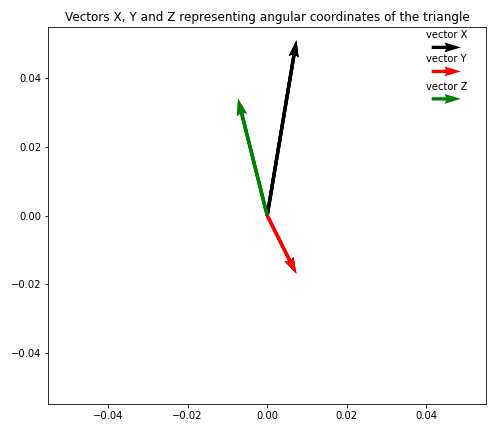
\includegraphics[scale=0.4]{Vectors_Fig.png}
	\caption{Plot representing the triangle formed by angular coordinates}
\end{figure}
\begin{align}
\begin{split}
\vec{X-Y} & = \myvec{0\\2c} \\
& = \myvec{0\\16}
\end{split}
\label{eq7}
\end{align}
\begin{align}
\begin{split}
\vec{Y-Z} & = \myvec{2a\\b-2c} \\
& = \myvec{4\\-12}
\end{split}
\label{eq8}
\end{align}
\begin{align}
\begin{split}
\text{Area of Triangle} & = \frac{1}{2} \times 4ac \\
& = \frac{1}{2} \times 4 \times 2 \times 8 \\
& = 32 \text{ unit}^2
\end{split}
\label{eq9}
\end{align}
\begin{figure}[h]
	\centering
	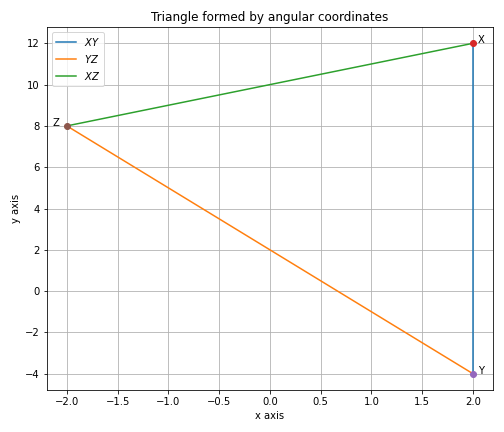
\includegraphics[scale=0.4]{Triangle_Fig.png}
	\caption{Plot representing the triangle formed by angular coordinates}
\end{figure}

\end{document}